\documentclass[a4paper, 11pt, twocolumn]{article}

\usepackage[czech]{babel}
\usepackage[utf8]{inputenc}
\usepackage[IL2]{fontenc}
\usepackage[left=1.5cm, top=2.5cm, text={18cm, 25cm}]{geometry}

\usepackage{times}
\usepackage{amsthm}
\usepackage{amssymb}
\usepackage{amsmath}
\usepackage{stackrel}
\usepackage{graphicx}

\graphicspath{{./img/}}



\begin{document}

	\begin{titlepage}
		\begin{center}
			{\Huge\textsc{Fakulta informačních technologií \\ \vspace*{0.2cm} Vysoké učení technické v~Brně}}\\
			\vspace{\stretch{0.382}} 
			\huge {Specifikace zadání a uživatelských požadavků} \\
			\Large {Tvorba uživatelských rozhraní} \\
			\vspace{\stretch{0.618}}
		\end{center}

		\Large{\hfill Vojtěch Kališ (xkalis03)} \\
		\Large{2021 \hfill Jan Lutonský (xluton02)}
	\end{titlepage}
	
	\twocolumn[{\centering{\Large \textbf{Individuální průzkum}\par}
	{\large Vojtěch Kališ, xkalis03@stud.fit.vutbr.cz\par}}
	\par\vspace*{0.8cm}]

	\section*{\large{Téma -- mobilní aplikace Time Planner}}
	\vspace*{-0.2cm}
	Jakožto téma jsem se rozhodl vybrat nějakou aplikaci, jejíž funkcionalita spočívá ve vytváření plánů, upomínek či jakéhokoliv jiného druhu poznámek za
	účelem zapsání si či připomenutí důležité události, schůze, nebo i~trivialit jako co je potřeba koupit při příští návštěvě obchodu apod.; čili jakýkoliv 
	například digitální kalendář, poznámkový blok a~jiné aplikace umožňující výše popsané. Zároveň proběhla snaha najít takovou aplikaci, na níž byly na
	první pohled patrné chyby z~pohledu GUI a~uživatelského procesu, a~to za účelem zjednodušení analýzy problémů dané aplikace a~následného návrhu
	jejich řešení.
	
	\section*{\large{Způsob zkoumání uživatele}}
	\vspace*{-0.2cm}
	Jako subjekt pro svůj uživatelský průzkum jsem si vybral svého bratra, jemuž jsem aplikaci na chvíli předal a~následně jej podrobil několika předem 
	přichystaným stručným otázkám, které měly za účel zjistit jeho pocity z aplikace, připomínky, požadavky a jiné.

	\section*{\large{Požadavky uživatele}} 
	\vspace*{-0.2cm}
	\begin{itemize}
		\item Přehlednost
		\vspace{-0.2cm}
		\item Jednoduchost použití
		\vspace{-0.2cm}
		\item Není zapotřebí převeliké množství funkcí
		\vspace{-0.2cm}
		\item Možnost změny barevného scématu a~pozadí
		\vspace{-0.2cm}
		\item Rychlá editace položek
	\end{itemize}

	\section*{\large{Způsob používání současné aplikace}}
	\vspace*{-0.2cm}
	Momentální aplikace je založena na třídění všech nových i~již vytvořených úloh do skupin podle různých kondicí, převážně pak tedy místa jejich vykonání, 
	čili např. na poznámky vytvořené pro školu, práci, na doma, volný čas a~tak dále. Postrádá možnost zobrazit je všechny chronologicky za sebou a~tím
	zbytečně vytváří zmatek, což jde proti jejímu účelu. Ihned po prvotním spuštění aplikace na uživatele vyskočí několikakrokový tutoriál na vytvoření nové
	úlohy, načež je uživatel stejně zmaten co to vlastně vytvořil a~proč, a~poté navíc zjistí že jej čeká ještě zkouknout dalších 10 tutoriálů. Odhaduji, že 
	právě v~tenhle moment by to obvyklý uživatel vzdal a~aplikaci zavřel, čemuž napovídá i~nepěkné hodnocení aplikace.


	\section*{\large{Identifikované potíže}}
	\vspace*{-0.2cm}
	\begin{itemize}
		\item Aplikace má zbytečně příliš mnoho funkcí, což ji dělá nepřehlednou a~komplikovanou
		\vspace{-0.2cm}
		\item Pouze dvě barevná schémata, skoro žádné možnosti kustomizace
		\vspace{-0.2cm}
		\item Zákazník očekává jednoduché řešení jednoduchého problému, ale čeká na něj složité monstrum
	\end{itemize}

	\section*{\large{\centering Vlastní návrh nového řešení}}
	\vspace*{-0.2cm}
	Aplikace má v hlavním panelu nástrojů pouze tři hlavní funkce, a~to konkrétně funkci pro vytvoření úlohy, zobrazení kalendáře s podrobnostmi k úlohám 
	v~následujících dnech a~také možnost grafického přepnutí mezi více režimy zobrazení úloh, přesně v tomto pořadí. Vytvořené úlohy obsahují v~hlavním 
	menu pouze jejich jméno a~čas konání, přičemž je možná každou úlohu rozkliknout, což otevře textový editor v~němž je možné i~doplnit přiblíženější 
	specifikaci k~dané ploze. V~pravém rohu položky je také tlačítko, které po rozkliknutí otevře jednoduché drop-down menu s možnostmi přejmenování 
	položky, nastavení upomínky a~nebo odstranění položky. V~pravém horním rohu menu je tlačítko jejž rozkliknutí otevře Nastavení, kde je dále 
	umožněno například měnit barevné schéma aplikace výběrem z~RGB palety, změnit používaný jazyk, nastavení zvuku apod.
	\vspace*{-0.1cm}
	\begin{center}
	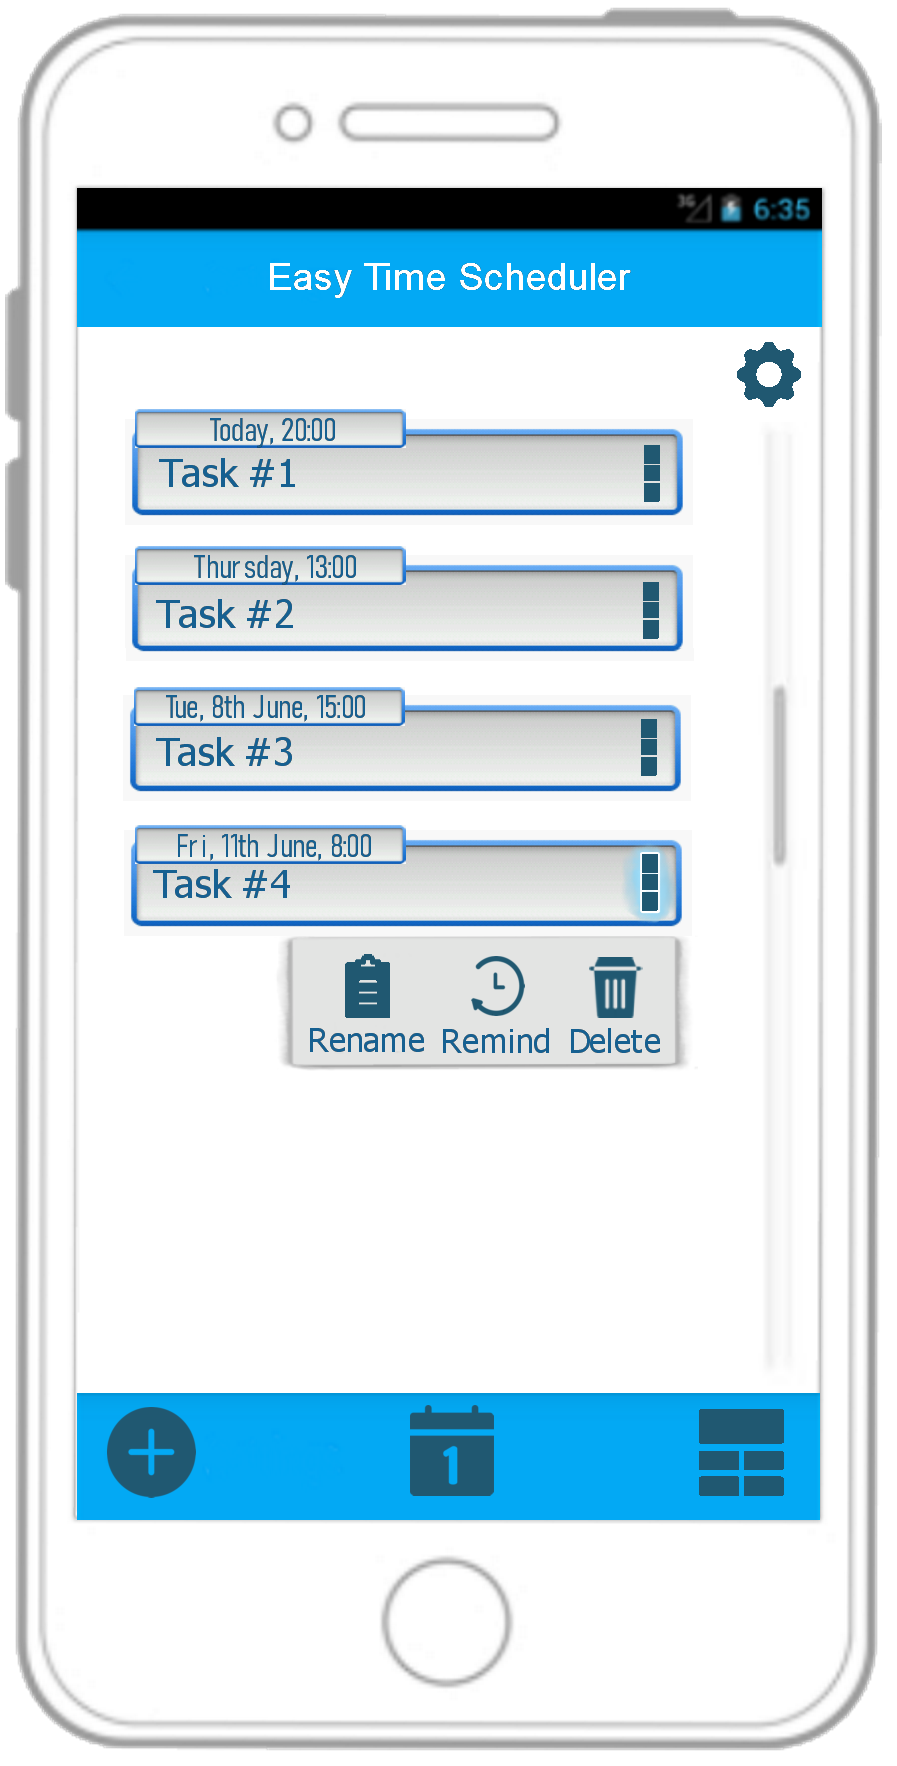
\includegraphics[width=0.34\textwidth]{timeplanner}
	\end{center}

	\newpage


	\twocolumn[{\centering{\Large \textbf{Individuální průzkum}\par}
	{\large Jan Lutonský, xluton02@stud.fit.vutbr.cz\par}}
	\par\vspace*{0.8cm}]

	\section*{Téma -- školní informační systém}
	
	
	\section*{Způsob zkoumání uživatele}

	\section*{Požadavky uživatele}

	\section*{Způsob používání současné aplikace}

	\section*{Identifikované potíže}

	\section*{Vlastní návrh nového řešení}


	\newpage


	\twocolumn[{\centering{\huge \textbf{Specifikace zadání a uživatelských požadavků}\par}
	{\Large téma Školní informační systém\par}}
	\par\vspace*{0.8cm}]

	
	\section*{wow}	

\end{document}